\documentclass[]{article}
\usepackage{lmodern}
\usepackage{amssymb,amsmath}
\usepackage{ifxetex,ifluatex}
\usepackage{fixltx2e} % provides \textsubscript
\ifnum 0\ifxetex 1\fi\ifluatex 1\fi=0 % if pdftex
  \usepackage[T1]{fontenc}
  \usepackage[utf8]{inputenc}
\else % if luatex or xelatex
  \ifxetex
    \usepackage{mathspec}
  \else
    \usepackage{fontspec}
  \fi
  \defaultfontfeatures{Ligatures=TeX,Scale=MatchLowercase}
\fi
% use upquote if available, for straight quotes in verbatim environments
\IfFileExists{upquote.sty}{\usepackage{upquote}}{}
% use microtype if available
\IfFileExists{microtype.sty}{%
\usepackage{microtype}
\UseMicrotypeSet[protrusion]{basicmath} % disable protrusion for tt fonts
}{}
\usepackage[margin=1in]{geometry}
\usepackage{hyperref}
\hypersetup{unicode=true,
            pdftitle={Mining Hamlet},
            pdfauthor={Rafa},
            pdfborder={0 0 0},
            breaklinks=true}
\urlstyle{same}  % don't use monospace font for urls
\usepackage{color}
\usepackage{fancyvrb}
\newcommand{\VerbBar}{|}
\newcommand{\VERB}{\Verb[commandchars=\\\{\}]}
\DefineVerbatimEnvironment{Highlighting}{Verbatim}{commandchars=\\\{\}}
% Add ',fontsize=\small' for more characters per line
\usepackage{framed}
\definecolor{shadecolor}{RGB}{248,248,248}
\newenvironment{Shaded}{\begin{snugshade}}{\end{snugshade}}
\newcommand{\AlertTok}[1]{\textcolor[rgb]{0.94,0.16,0.16}{#1}}
\newcommand{\AnnotationTok}[1]{\textcolor[rgb]{0.56,0.35,0.01}{\textbf{\textit{#1}}}}
\newcommand{\AttributeTok}[1]{\textcolor[rgb]{0.77,0.63,0.00}{#1}}
\newcommand{\BaseNTok}[1]{\textcolor[rgb]{0.00,0.00,0.81}{#1}}
\newcommand{\BuiltInTok}[1]{#1}
\newcommand{\CharTok}[1]{\textcolor[rgb]{0.31,0.60,0.02}{#1}}
\newcommand{\CommentTok}[1]{\textcolor[rgb]{0.56,0.35,0.01}{\textit{#1}}}
\newcommand{\CommentVarTok}[1]{\textcolor[rgb]{0.56,0.35,0.01}{\textbf{\textit{#1}}}}
\newcommand{\ConstantTok}[1]{\textcolor[rgb]{0.00,0.00,0.00}{#1}}
\newcommand{\ControlFlowTok}[1]{\textcolor[rgb]{0.13,0.29,0.53}{\textbf{#1}}}
\newcommand{\DataTypeTok}[1]{\textcolor[rgb]{0.13,0.29,0.53}{#1}}
\newcommand{\DecValTok}[1]{\textcolor[rgb]{0.00,0.00,0.81}{#1}}
\newcommand{\DocumentationTok}[1]{\textcolor[rgb]{0.56,0.35,0.01}{\textbf{\textit{#1}}}}
\newcommand{\ErrorTok}[1]{\textcolor[rgb]{0.64,0.00,0.00}{\textbf{#1}}}
\newcommand{\ExtensionTok}[1]{#1}
\newcommand{\FloatTok}[1]{\textcolor[rgb]{0.00,0.00,0.81}{#1}}
\newcommand{\FunctionTok}[1]{\textcolor[rgb]{0.00,0.00,0.00}{#1}}
\newcommand{\ImportTok}[1]{#1}
\newcommand{\InformationTok}[1]{\textcolor[rgb]{0.56,0.35,0.01}{\textbf{\textit{#1}}}}
\newcommand{\KeywordTok}[1]{\textcolor[rgb]{0.13,0.29,0.53}{\textbf{#1}}}
\newcommand{\NormalTok}[1]{#1}
\newcommand{\OperatorTok}[1]{\textcolor[rgb]{0.81,0.36,0.00}{\textbf{#1}}}
\newcommand{\OtherTok}[1]{\textcolor[rgb]{0.56,0.35,0.01}{#1}}
\newcommand{\PreprocessorTok}[1]{\textcolor[rgb]{0.56,0.35,0.01}{\textit{#1}}}
\newcommand{\RegionMarkerTok}[1]{#1}
\newcommand{\SpecialCharTok}[1]{\textcolor[rgb]{0.00,0.00,0.00}{#1}}
\newcommand{\SpecialStringTok}[1]{\textcolor[rgb]{0.31,0.60,0.02}{#1}}
\newcommand{\StringTok}[1]{\textcolor[rgb]{0.31,0.60,0.02}{#1}}
\newcommand{\VariableTok}[1]{\textcolor[rgb]{0.00,0.00,0.00}{#1}}
\newcommand{\VerbatimStringTok}[1]{\textcolor[rgb]{0.31,0.60,0.02}{#1}}
\newcommand{\WarningTok}[1]{\textcolor[rgb]{0.56,0.35,0.01}{\textbf{\textit{#1}}}}
\usepackage{graphicx,grffile}
\makeatletter
\def\maxwidth{\ifdim\Gin@nat@width>\linewidth\linewidth\else\Gin@nat@width\fi}
\def\maxheight{\ifdim\Gin@nat@height>\textheight\textheight\else\Gin@nat@height\fi}
\makeatother
% Scale images if necessary, so that they will not overflow the page
% margins by default, and it is still possible to overwrite the defaults
% using explicit options in \includegraphics[width, height, ...]{}
\setkeys{Gin}{width=\maxwidth,height=\maxheight,keepaspectratio}
\IfFileExists{parskip.sty}{%
\usepackage{parskip}
}{% else
\setlength{\parindent}{0pt}
\setlength{\parskip}{6pt plus 2pt minus 1pt}
}
\setlength{\emergencystretch}{3em}  % prevent overfull lines
\providecommand{\tightlist}{%
  \setlength{\itemsep}{0pt}\setlength{\parskip}{0pt}}
\setcounter{secnumdepth}{0}
% Redefines (sub)paragraphs to behave more like sections
\ifx\paragraph\undefined\else
\let\oldparagraph\paragraph
\renewcommand{\paragraph}[1]{\oldparagraph{#1}\mbox{}}
\fi
\ifx\subparagraph\undefined\else
\let\oldsubparagraph\subparagraph
\renewcommand{\subparagraph}[1]{\oldsubparagraph{#1}\mbox{}}
\fi

%%% Use protect on footnotes to avoid problems with footnotes in titles
\let\rmarkdownfootnote\footnote%
\def\footnote{\protect\rmarkdownfootnote}

%%% Change title format to be more compact
\usepackage{titling}

% Create subtitle command for use in maketitle
\newcommand{\subtitle}[1]{
  \posttitle{
    \begin{center}\large#1\end{center}
    }
}

\setlength{\droptitle}{-2em}

  \title{Mining Hamlet}
    \pretitle{\vspace{\droptitle}\centering\huge}
  \posttitle{\par}
    \author{Rafa}
    \preauthor{\centering\large\emph}
  \postauthor{\par}
      \predate{\centering\large\emph}
  \postdate{\par}
    \date{2018-01-20}


\begin{document}
\maketitle

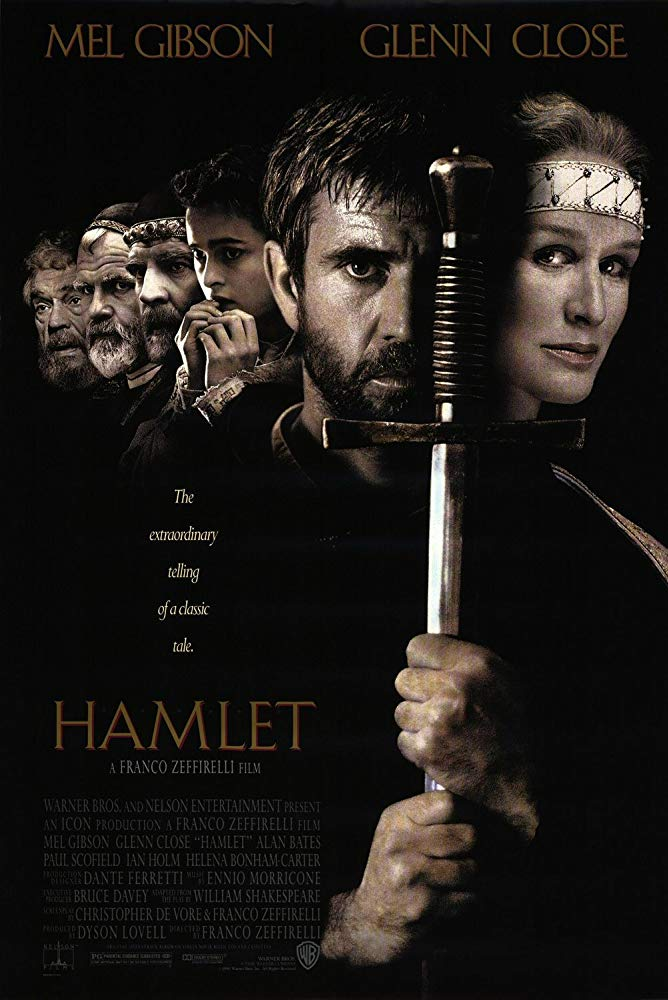
\includegraphics{/post/2018-08-20-hamlet_files/MV5BMjI5OTgwNTc3M15BMl5BanBnXkFtZTgwNDY1NTk4NjE@._V1_SY1000_CR0,0,668,1000_AL_.jpg}

A lot of Shakespeare's tragic heores don't dominate the first act of
their plays. Instead, other characters speak about them, setting the
scene for exploring their personalities later in the plays. This is the
case of Julius Caesar, Macbeth and Othello (but not of King Lear).

In this post I go over the text of Hamlet, Prince of Denmark, using the
quantity of lines spoken by character to visualize the dynamic of the
play. We'll get the chance to use \texttt{dplyr} and some
\texttt{regular\ expressions}.

\hypertarget{getting-the-text-of-the-plays}{%
\section{Getting the text of the
plays}\label{getting-the-text-of-the-plays}}

The text of Shakespeare's plays is available from the \texttt{gutenberg}
package. I downloaded the text and made it available as a data frame
\href{/post/2018-08-20-hamlet_files/shakespeare_plays.rds}{here} so you
don't have to.

\begin{Shaded}
\begin{Highlighting}[]
\NormalTok{books <-}\StringTok{ }\KeywordTok{readRDS}\NormalTok{(}\StringTok{'../../public/post/2018-08-20-hamlet_files/shakespeare_plays.rds'}\NormalTok{)}
\NormalTok{hamlet <-}\StringTok{ }\NormalTok{books }\OperatorTok\StringTok{  }
\StringTok{  }\KeywordTok{filter}\NormalTok{(title }\OperatorTok{==}\StringTok{ "Hamlet, Prince of Denmark"}\NormalTok{)}
\end{Highlighting}
\end{Shaded}

\hypertarget{extracting-the-character-names}{%
\section{Extracting the Character
names}\label{extracting-the-character-names}}

We can use a regular expressions to extract character names from the
lines of the play. Most characters names appear abreviated (Ham. for
Hamlet, Hor. for Horatio).

\texttt{lag} and \texttt{cumsum} are useful inside call to
\texttt{mutate} to look at consecutive lines in the data frame. I also
create a line number index with \texttt{row\_number}.

\begin{Shaded}
\begin{Highlighting}[]
\CommentTok{# Fran., Ham., Pol.}
\NormalTok{CHAR_REGEX <-}\StringTok{ }\KeywordTok{regex}\NormalTok{(}\StringTok{"^([A-Z][a-z]*)}\CharTok{\textbackslash{}\textbackslash{}}\StringTok{."}\NormalTok{)}
\CommentTok{# Stage Dir}
\CommentTok{# [Enter Horatio and Marcellus.]}
\NormalTok{STAGEDIR_REGEX <-}\StringTok{ }\KeywordTok{regex}\NormalTok{(}\StringTok{"(}\CharTok{\textbackslash{}\textbackslash{}}\StringTok{[.+}\CharTok{\textbackslash{}\textbackslash{}}\StringTok{])"}\NormalTok{)}

\NormalTok{hamlet <-}\StringTok{ }\NormalTok{hamlet }\OperatorTok\StringTok{ }
\StringTok{  }\KeywordTok{mutate}\NormalTok{(}\DataTypeTok{char_name =} \KeywordTok{str_match}\NormalTok{(text, CHAR_REGEX)[,}\DecValTok{2}\NormalTok{]) }\OperatorTok\StringTok{ }
\StringTok{  }\KeywordTok{mutate}\NormalTok{(}\DataTypeTok{stage_dir =} \KeywordTok{str_match}\NormalTok{(text, STAGEDIR_REGEX)[,}\DecValTok{2}\NormalTok{],}
         \DataTypeTok{char_name =} \KeywordTok{if_else}\NormalTok{(}\OperatorTok{!}\KeywordTok{is.na}\NormalTok{(stage_dir), }\StringTok{"director"}\NormalTok{, char_name)) }\OperatorTok
\StringTok{  }\KeywordTok{mutate}\NormalTok{(}\DataTypeTok{start_speech =} \OperatorTok{!}\KeywordTok{is.na}\NormalTok{(char_name) }\OperatorTok{&}\StringTok{ }
\StringTok{           }\KeywordTok{lag}\NormalTok{(text) }\OperatorTok{==}\StringTok{ ""}\NormalTok{) }\OperatorTok
\StringTok{  }\KeywordTok{mutate}\NormalTok{(}\DataTypeTok{speech_idx =} \KeywordTok{cumsum}\NormalTok{(start_speech)) }\OperatorTok\StringTok{ }
\StringTok{  }\KeywordTok{mutate}\NormalTok{(}\DataTypeTok{line =} \KeywordTok{row_number}\NormalTok{()) }\OperatorTok\StringTok{ }
\StringTok{  }\KeywordTok{select}\NormalTok{(text, char_name, start_speech, speech_idx, line)}
\end{Highlighting}
\end{Shaded}

Now we need to create a \texttt{data\ frame} of speeches. Each line is a
speech in the play, with the character that speaks it and the number of
lines it lasts.

\begin{Shaded}
\begin{Highlighting}[]

\CommentTok{# Build a df with speech, start line, length char}
\NormalTok{speeches_df <-}\StringTok{ }\NormalTok{hamlet }\OperatorTok\StringTok{ }
\StringTok{  }\KeywordTok{group_by}\NormalTok{(speech_idx) }\OperatorTok\StringTok{ }
\StringTok{  }\KeywordTok{summarise}\NormalTok{(}\DataTypeTok{char_name =} \KeywordTok{first}\NormalTok{(char_name), }
            \DataTypeTok{line =} \KeywordTok{first}\NormalTok{(line),}
          \DataTypeTok{speech_length =} \KeywordTok{as.integer}\NormalTok{(}\KeywordTok{n}\NormalTok{()}\OperatorTok{-}\DecValTok{2}\NormalTok{)) }\OperatorTok\StringTok{ }
\StringTok{  }\NormalTok{dplyr}\OperatorTok{::}\KeywordTok{filter}\NormalTok{(char_name }\OperatorTok{!=}\StringTok{ "director"}\NormalTok{)}
\end{Highlighting}
\end{Shaded}

The longest speech is by Hamlet (duh!), and starts at line 2677.

\begin{Shaded}
\begin{Highlighting}[]
\NormalTok{speeches_df }\OperatorTok\StringTok{ }
\StringTok{  }\KeywordTok{arrange}\NormalTok{(}\OperatorTok{-}\NormalTok{speech_length)}
\CommentTok{## # A tibble: 1,077 x 4}
\CommentTok{##    speech_idx char_name  line speech_length}
\CommentTok{##         <int> <chr>     <int>         <int>}
\CommentTok{##  1        498 Ham        2677            60}
\CommentTok{##  2        234 Ghost      1296            50}
\CommentTok{##  3         69 King        383            39}
\CommentTok{##  4        761 Ham        4039            36}
\CommentTok{##  5        154 Laer        846            35}
\CommentTok{##  6        522 Ham        2857            35}
\CommentTok{##  7        480 Pol        2553            34}
\CommentTok{##  8        479 Ham        2518            33}
\CommentTok{##  9        568 Ham        3139            32}
\CommentTok{## 10         84 King        502            31}
\CommentTok{## # ... with 1,067 more rows}
\end{Highlighting}
\end{Shaded}

Lets take a look at the text of the speech:

\begin{Shaded}
\begin{Highlighting}[]
\NormalTok{hamlet }\OperatorTok\StringTok{ }
\StringTok{  }\KeywordTok{filter}\NormalTok{(line }\OperatorTok\StringTok{ }\DecValTok{2677}\OperatorTok{:}\DecValTok{2690}\NormalTok{) }\OperatorTok\StringTok{ }
\StringTok{  }\KeywordTok{select}\NormalTok{(text) }
\CommentTok{## # A tibble: 14 x 1}
\CommentTok{##    text                                           }
\CommentTok{##    <chr>                                          }
\CommentTok{##  1 Ham.                                           }
\CommentTok{##  2 Ay, so, God b' wi' ye!                         }
\CommentTok{##  3 Now I am alone.                                }
\CommentTok{##  4 O, what a rogue and peasant slave am I!        }
\CommentTok{##  5 Is it not monstrous that this player here,     }
\CommentTok{##  6 But in a fiction, in a dream of passion,       }
\CommentTok{##  7 Could force his soul so to his own conceit     }
\CommentTok{##  8 That from her working all his visage wan'd;    }
\CommentTok{##  9 Tears in his eyes, distraction in's aspect,    }
\CommentTok{## 10 A broken voice, and his whole function suiting }
\CommentTok{## 11 With forms to his conceit? And all for nothing!}
\CommentTok{## 12 For Hecuba?                                    }
\CommentTok{## 13 What's Hecuba to him, or he to Hecuba,         }
\CommentTok{## 14 That he should weep for her? What would he do,}
\end{Highlighting}
\end{Shaded}

Lets focus on the characters with the most lines:

\begin{Shaded}
\begin{Highlighting}[]
\NormalTok{top_speakers <-}\StringTok{ }\NormalTok{speeches_df }\OperatorTok\StringTok{ }
\StringTok{  }\KeywordTok{group_by}\NormalTok{(char_name)  }\OperatorTok
\StringTok{  }\KeywordTok{summarize}\NormalTok{(}\DataTypeTok{total_lines =} \KeywordTok{sum}\NormalTok{(speech_length)) }\OperatorTok\StringTok{ }
\StringTok{  }\KeywordTok{arrange}\NormalTok{(}\OperatorTok{-}\NormalTok{total_lines) }\OperatorTok\StringTok{ }
\StringTok{  }\KeywordTok{head}\NormalTok{(}\DecValTok{6}\NormalTok{)}
\end{Highlighting}
\end{Shaded}

Use \texttt{inner\_join} to discard the less important characters:

\begin{Shaded}
\begin{Highlighting}[]
\CommentTok{# Keep speeches by these speakers}
\NormalTok{speeches_df_main <-}\StringTok{ }\NormalTok{speeches_df }\OperatorTok\StringTok{ }
\StringTok{  }\KeywordTok{inner_join}\NormalTok{(top_speakers, }\DataTypeTok{by =} \StringTok{"char_name"}\NormalTok{) }\OperatorTok\StringTok{ }
\StringTok{  }\KeywordTok{filter}\NormalTok{(}\OperatorTok{!}\KeywordTok{is.na}\NormalTok{(char_name))}
\end{Highlighting}
\end{Shaded}

The last thing we need is a column with the cumulative lines spoken by
each character:

\begin{Shaded}
\begin{Highlighting}[]
\NormalTok{speeches_df_main <-}\StringTok{ }\NormalTok{speeches_df_main }\OperatorTok\StringTok{ }
\StringTok{   }\KeywordTok{group_by}\NormalTok{(char_name) }\OperatorTok\StringTok{ }
\StringTok{   }\KeywordTok{mutate}\NormalTok{(}\DataTypeTok{cum_lines =} \KeywordTok{as.integer}\NormalTok{(}\KeywordTok{cumsum}\NormalTok{(speech_length))) }\OperatorTok\StringTok{ }
\StringTok{   }\KeywordTok{ungroup}\NormalTok{() }\OperatorTok\StringTok{ }
\StringTok{   }\KeywordTok{mutate}\NormalTok{(}\DataTypeTok{char_name =} \KeywordTok{fct_recode}\NormalTok{(char_name,}
             \StringTok{"Horatio"}\NormalTok{       =}\StringTok{ "Hor"}\NormalTok{,}
             \StringTok{"King Claudius"}\NormalTok{ =}\StringTok{ "King"}\NormalTok{,}
             \StringTok{"Laertes"}\NormalTok{       =}\StringTok{ "Laer"}\NormalTok{,}
             \StringTok{"Polonius"}\NormalTok{      =}\StringTok{ "Pol"}\NormalTok{,}
             \StringTok{"Ophelia"}\NormalTok{       =}\StringTok{ "Oph"}\NormalTok{,}
             \StringTok{"Hamlet"}\NormalTok{        =}\StringTok{ "Ham"}\NormalTok{))}
\end{Highlighting}
\end{Shaded}

Now we can plot the play:

\begin{Shaded}
\begin{Highlighting}[]
\CommentTok{# color palette}
\NormalTok{col.pal <-}\StringTok{ }\NormalTok{RColorBrewer}\OperatorTok{::}\KeywordTok{brewer.pal}\NormalTok{(}\DecValTok{8}\NormalTok{, }\StringTok{"Set2"}\NormalTok{)}

\CommentTok{# Plot Play}
\NormalTok{g <-}\StringTok{ }\KeywordTok{ggplot}\NormalTok{(speeches_df_main, }\KeywordTok{aes}\NormalTok{(line, cum_lines, }\DataTypeTok{fill =}\NormalTok{ char_name)) }\OperatorTok{+}\StringTok{ }
\StringTok{  }\KeywordTok{guides}\NormalTok{(}\DataTypeTok{colour =} \KeywordTok{guide_legend}\NormalTok{(}\DataTypeTok{title =} \OtherTok{NULL}\NormalTok{)) }\OperatorTok{+}
\StringTok{  }\KeywordTok{geom_area}\NormalTok{(}\DataTypeTok{alpha =} \FloatTok{0.8}\NormalTok{) }\OperatorTok{+}\StringTok{ }
\StringTok{  }\KeywordTok{guides}\NormalTok{(}\DataTypeTok{fill =} \KeywordTok{guide_legend}\NormalTok{(}\DataTypeTok{title =} \OtherTok{NULL}\NormalTok{)) }\OperatorTok{+}
\StringTok{  }\KeywordTok{scale_fill_brewer}\NormalTok{(}\DataTypeTok{palette =} \StringTok{"Set2"}\NormalTok{) }\OperatorTok{+}\StringTok{ }
\StringTok{  }\KeywordTok{labs}\NormalTok{(}\DataTypeTok{title =} \StringTok{"Cumulative lines"}\NormalTok{, }\DataTypeTok{subtitle =} \StringTok{"By Character"}\NormalTok{) }\OperatorTok{+}\StringTok{ }
\StringTok{  }\KeywordTok{xlab}\NormalTok{(}\StringTok{"Line"}\NormalTok{) }\OperatorTok{+}\StringTok{ }
\StringTok{  }\KeywordTok{ylab}\NormalTok{(}\StringTok{"Spoken Lines"}\NormalTok{) }\OperatorTok{+}
\StringTok{  }\KeywordTok{theme_bw}\NormalTok{() }\OperatorTok{+}\StringTok{ }
\StringTok{  }\KeywordTok{theme}\NormalTok{(}\DataTypeTok{plot.title =} \KeywordTok{element_text}\NormalTok{(}\DataTypeTok{hjust =} \FloatTok{0.5}\NormalTok{),}
        \DataTypeTok{plot.subtitle =} \KeywordTok{element_text}\NormalTok{(}\DataTypeTok{hjust =} \FloatTok{0.5}\NormalTok{),}
        \DataTypeTok{panel.border =} \KeywordTok{element_blank}\NormalTok{()) }\OperatorTok{+}
\StringTok{  }\KeywordTok{scale_x_continuous}\NormalTok{(}\DataTypeTok{expand =} \KeywordTok{c}\NormalTok{(}\DecValTok{0}\NormalTok{, }\DecValTok{0}\NormalTok{)) }\OperatorTok{+}\StringTok{ }
\StringTok{  }\KeywordTok{scale_y_continuous}\NormalTok{(}\DataTypeTok{expand =} \KeywordTok{c}\NormalTok{(}\DecValTok{0}\NormalTok{, }\DecValTok{0}\NormalTok{))}

\NormalTok{g}
\end{Highlighting}
\end{Shaded}

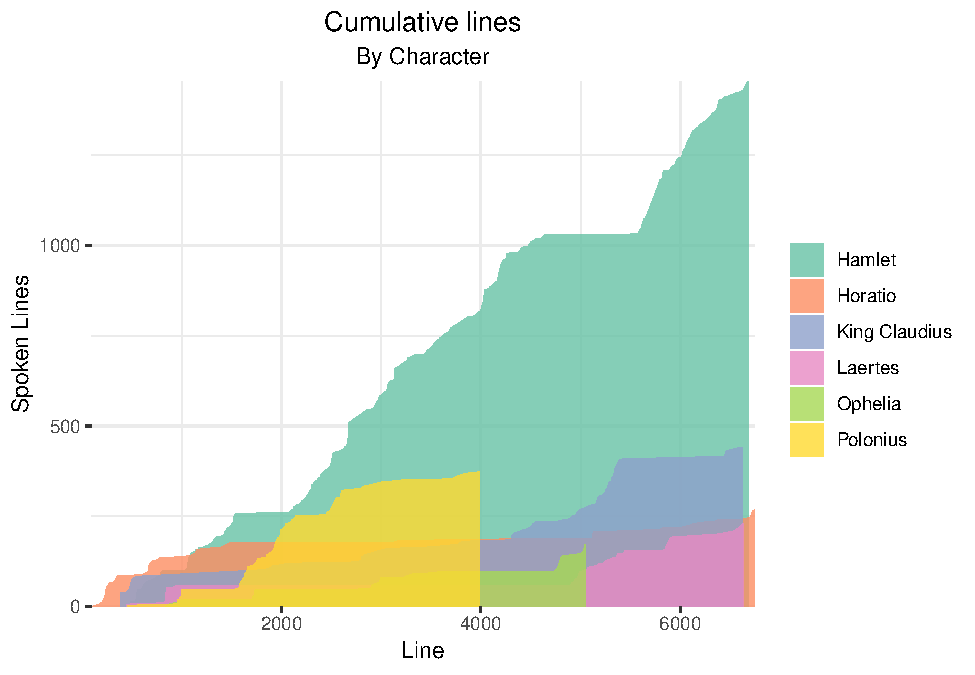
\includegraphics{2018-08-20-hamlet_files/figure-latex/unnamed-chunk-9-1.pdf}

The plot shows the dynamic of the play quite nicely. Horatio, Hamlet's
friend figures quite prominenty at the beggining.

Polonius has a lot of lines in the middle of the play, until he's caught
behind the arras just before line 4000.

Hamlet eats up the whole play towards the end in his stand of against
evil King Claudius.


\end{document}
